% !TeX root = ../BA_LateXVorlage.tex
\section{Grundlagen}
Im folgenden Kapitel werden die theoretischen und technischen Grundlagen erklärt, die für das Verständnis der Funktionsweise von MultiTextCompare notwendig sind.

\subsection{String similarity Algorithmen}\label{String similarity Algorithmen}
Für eine Software, die dazu dient textbasierte Dateien miteinander zu vergleichen ist es essenziell eine Metrik zu finden, die die Ähnlichkeit von Zeichenketten (engl. Strings) bewerten kann. Allerdings ist der Begriff der Ähnlichkeit im allgemeinen Sprachgebrauch ein subjektives Konstrukt. Der Begriff der Gleichheit scheint hingegen auf den ersten Blick etwas greifbarer.
Strings sind gleich, wenn ihre Länge, ihre Zeichen und die Reihenfolge dieser Zeichen gleich sind. In der Sprache existieren allerdings auch Wörter, die bei gleicher Schreibweise unterschiedliche Bedeutungen haben. Wörter sind hierbei im strukturellen Sinne auch nur durch Leerzeichen voneinander getrennte Strings mit Zeichen des zugehörigen Alphabets. Im Deutschen kann z.B. das Wort \glqq einstellen\grqq{} je nach Kontext u.a. die Bedeutung \glqq mit einer Tätigkeit [...] aufhören\grqq{}, \glqq etwas regulieren\grqq{}  und \glqq (jemanden) in ein Arbeitsverhältnis nehmen \grqq{} haben \autocite{dudenEinstellen}, obwohl sich die Schreibweise nicht ändert. Andersherum gibt es Wörter, die anders geschrieben werden und dennoch die gleiche Bedeutung haben. Je nach Kontext können z.B. die Wörter Software, Anwendung und System auf den gleichen Begriff angewandt werden.

Diese Inkonsistenzen sind allerdings schwer messbar und treten zudem bei automatisiert generierten Dateien selten auf, weshalb bei MultiTextCompare auf einen rein strukturellen Vergleich von Strings gesetzt wird. Im Folgenden werden zwei verbreitete Algorithmen für den Vergleich von Strings vorgestellt.

\subsubsection{Longest common subsequence}\label{lcs}

Die \acrfull{lcs} für zwei Strings ist die größte Menge aller Zeichen, die in beiden Strings in gleicher Reihenfolge vorkommen. Diese Menge wird durch Löschung einzelner Zeichen der beiden Strings errechnet, sodass beide Strings nun dieser Menge entsprechen \autocite[]{lcsFirstArticle}. Dadurch dass die Strings nicht gleich lang sein müssen, können Zeichen der Ergebnismenge nicht für beide Strings an den gleichen Indices stehen.

Das folgende Beispiel zeigt zwei unterschiedliche Strings $S_1$ und $S_2$ für die die \acrshort{lcs} berechnet werden soll, wobei unterschiedliche Zeichen in rot markiert sind.

\[ S_1 = \color{black} D \color{red}ie \color{black}s \ ist \ ein \ Text\]
\[ S_2 = D\color{red}a\color{black}s \  ist \  ein  \ \color{red}anderer\color{black} \ Text\]

Die zugehörige Ergebnismenge $M_{LCS}$ ist $ \{Ds \ ist \ ein \ Text\}$. Der \acrshort{lcs} Algorithmus findet Verwendung bei der Erstellung der \acrfull{diff}, einem Verfahren bei dem die Unterschiede zwischen zwei Dateien ermittelt werden. Die Versionskontroll-Software Git, ermittelt bspw. die \acrshort{diff} für verschiedene Versionen der gleichen Datei. Dafür wird grundsätzlich der \acrshort{lcs}-Algorithmus verwendet \autocite{diffLCS}.

Die Implementierung der \acrshort{diff} in der Software MultiTextCompare beruht für zwei Dateien ebenfalls auf dem gleichen Prinzip. Dort entsteht für zwei Dateien $A $ und $B$ genau ein Vergleichsdurchlauf $D_2 = \{A,B\}$, für den alle Zeilen von $A$ und $B$ mittels der \acrshort{lcs} miteinander verglichen werden. Zeichen, die sich in der Ergebnismenge $M_{LCS}$ befinden, werden im \acrfull{ui} als unverändert (weiß) dargestellt, gelöschte und eingefügte Zeichen werden entsprechend rot und grün markiert.
Für drei Dateien $A$, $B$, $C$ wird weiterhin die \acrshort{lcs} verwendet, allerdings entstehen dort 3 Vergleichsdurchläufe $D_3 = \{ \{A,B\}, \{A,C\}, \{B,C\} \}$. Dieses Verhalten wird im Vergleich zu alternativer Software in Kapitel 3.1 genauer beleuchtet. 

Eine weitere interessante Metrik ist die Länge der LCS (LLCS). Diese entspricht für das Beispiel oben $|M_{LCS}| = 15$ und gilt als sinnvolle Quantifizierung der Ähnlichkeit von zwei oder mehr Strings. Als Metrik ist sie auch verwandt zur \textit{Edit Distance}, der minimalen Anzahl an Einfügungen, Löschungen und Änderungen von Zeichen um einen String in einen anderen zu überführen \autocite{llcs}. Im Gegensatz zur Edit Distance beschreibt die \acrshort{llcs} allerdings die Anzahl der \textit{gemeinsamen} Zeichen. Die beiden Begriffe sind also zu einem gewissen Grad komplementär.

% HIER NOCH ETWAS DAZU EINFÜGEN DASS NUR INSERTS UND DELETIONS ERLAUBT SIND ?

Auch die \acrshort{llcs} wird innerhalb von MultiTextCompare verwendet. Durch sie wird im \acrshort{diff}-Prozess festgestellt ob zwei Strings eine Mindestähnlichkeit erfüllen um zu entscheiden, ob gleiche Zeichen noch als gleich geblieben angezeigt werden sollen oder die zwei Strings eine komplette Zeilenlöschung bzw. Zeileneinfügung repräsentieren.

Damit ähnliche, aber verschobene Zeilen miteinander für die \acrshort{diff} verglichen werden können, existiert ein Matcher, der innerhalb der zu vergleichenden Dateien nach ähnlichen Zeilen sucht um diese an den selben Zeilenindex zu schreiben. Für die jeweiligen Strings $S_1, S_2$ zweier nichtleerer Zeilen $Z_1, Z_2$ existiert genau dann ein Match $M$ wenn

\begin{equation}
    \acrshort{llcs}(S_1,S_2) \geq (max(|S_1|, |S_2| ) \cdot x), \ mit \ 0 \leq x \leq 1
    \label{eq:matchat}
\end{equation}

gilt, wobei $x$ ein vom Benutzer einstellbarer Ähnlichkeitsfaktor ist. 


\subsubsection{Levenshtein-Distanz}\label{Levenshtein-Distanz}

Die Levenshtein-Distanz, benannt nach dem russischen Mathematiker Vladimir Levenshtein, ist eine weitere verbreitete Form der Edit Distance. Im Gegensatz zur \acrshort{llcs} beschreibt sie nun tatsächlich die minimale Anzahl an Operationen um Strings ineinander zu überführen und nicht mehr wie ähnlich sich zwei Strings sind. Als kleines Beispiel wird in Abb. \ref{fig:editDist} die Transformation des Wortes \glqq Geschenk\grqq{} in \glqq Gebiet\grqq{} vorgeführt. Ein orangener Knoten symbolisiert eine Änderung und ein roter Knoten steht für eine Löschung und ein dicker, schwarzer Rand kennzeichnet ein unverändertes Zeichen. Dabei ergibt sich für die beiden Strings eine Edit Distance von 5 und ist damit gleich der Anzahl der unterschiedlichen, farbigen Knoten.

\begin{figure}
    %Original
\begin{tikzpicture}[roundnode/.style={circle, draw=black, fill=white, semithick, minimum size=7mm},
currentnode/.style={circle, draw=black, fill=white, very thick, minimum size=7mm}]
\node[roundnode] (g) {G};
\node[roundnode] (e1) [right=of g] {e};
\node[roundnode] (s) [right=of e1] {s};
\node[roundnode] (c) [right=of s] {c};
\node[roundnode] (h) [right=of c] {h};
\node[roundnode] (e2) [right=of h] {e};
\node[roundnode] (n) [right=of e2] {n};
\node[roundnode] (k) [right=of n] {k};

\draw[->] (g.east) -- (e1.west);
\draw[->] (e1.east) -- (s.west);
\draw[->] (s.east) -- (c.west);
\draw[->] (c.east) -- (h.west);
\draw[->] (h.east) -- (e2.west);
\draw[->] (e2.east) -- (n.west);
\draw[->] (n.east) -- (k.west);
\end{tikzpicture}

\begin{tikzpicture}[roundnode/.style={circle, draw=black, fill=white, semithick, minimum size=7mm},
currentnode/.style={circle, draw=black, fill=white, very thick, minimum size=7mm}]
\node[currentnode] (g) {G};
\node[roundnode] (e1) [right=of g] {e};
\node[roundnode] (s) [right=of e1] {s};
\node[roundnode] (c) [right=of s] {c};
\node[roundnode] (h) [right=of c] {h};
\node[roundnode] (e2) [right=of h] {e};
\node[roundnode] (n) [right=of e2] {n};
\node[roundnode] (k) [right=of n] {k};

\draw[->] (g.east) -- (e1.west);
\draw[->] (e1.east) -- (s.west);
\draw[->] (s.east) -- (c.west);
\draw[->] (c.east) -- (h.west);
\draw[->] (h.east) -- (e2.west);
\draw[->] (e2.east) -- (n.west);
\draw[->] (n.east) -- (k.west);
\end{tikzpicture}

\begin{tikzpicture}[roundnode/.style={circle, draw=black, fill=white, semithick, minimum size=7mm},
currentnode/.style={circle, draw=black, fill=white, very thick, minimum size=7mm}]
\node[currentnode] (g) {G};
\node[currentnode] (e1) [right=of g] {e};
\node[roundnode] (s) [right=of e1] {s};
\node[roundnode] (c) [right=of s] {c};
\node[roundnode] (h) [right=of c] {h};
\node[roundnode] (e2) [right=of h] {e};
\node[roundnode] (n) [right=of e2] {n};
\node[roundnode] (k) [right=of n] {k};

\draw[->] (g.east) -- (e1.west);
\draw[->] (e1.east) -- (s.west);
\draw[->] (s.east) -- (c.west);
\draw[->] (c.east) -- (h.west);
\draw[->] (h.east) -- (e2.west);
\draw[->] (e2.east) -- (n.west);
\draw[->] (n.east) -- (k.west);
\end{tikzpicture}

\begin{tikzpicture}[roundnode/.style={circle, draw=black, fill=white, semithick, minimum size=7mm},
currentnode/.style={circle, draw=black, fill=white, very thick, minimum size=7mm},
replacenode/.style={circle, draw=orange, fill=white, very thick, minimum size=7mm}]
\node[currentnode] (g) {G};
\node[currentnode] (e1) [right=of g] {e};
\node[replacenode] (s) [right=of e1] {b};
\node[roundnode] (c) [right=of s] {c};
\node[roundnode] (h) [right=of c] {h};
\node[roundnode] (e2) [right=of h] {e};
\node[roundnode] (n) [right=of e2] {n};
\node[roundnode] (k) [right=of n] {k};

\draw[->] (g.east) -- (e1.west);
\draw[->] (e1.east) -- (s.west);
\draw[->] (s.east) -- (c.west);
\draw[->] (c.east) -- (h.west);
\draw[->] (h.east) -- (e2.west);
\draw[->] (e2.east) -- (n.west);
\draw[->] (n.east) -- (k.west);
\end{tikzpicture}

\begin{tikzpicture}[roundnode/.style={circle, draw=black, fill=white, semithick, minimum size=7mm},
currentnode/.style={circle, draw=black, fill=white, very thick, minimum size=7mm},
replacenode/.style={circle, draw=orange, fill=white, very thick, minimum size=7mm}]
\node[currentnode] (g) {G};
\node[currentnode] (e1) [right=of g] {e};
\node[replacenode] (s) [right=of e1] {b};
\node[replacenode] (c) [right=of s] {i};
\node[roundnode] (h) [right=of c] {h};
\node[roundnode] (e2) [right=of h] {e};
\node[roundnode] (n) [right=of e2] {n};
\node[roundnode] (k) [right=of n] {k};

\draw[->] (g.east) -- (e1.west);
\draw[->] (e1.east) -- (s.west);
\draw[->] (s.east) -- (c.west);
\draw[->] (c.east) -- (h.west);
\draw[->] (h.east) -- (e2.west);
\draw[->] (e2.east) -- (n.west);
\draw[->] (n.east) -- (k.west);
\end{tikzpicture}

\begin{tikzpicture}[roundnode/.style={circle, draw=black, fill=white, semithick, minimum size=7mm},
currentnode/.style={circle, draw=black, fill=white, very thick, minimum size=7mm},
replacenode/.style={circle, draw=orange, fill=white, very thick, minimum size=7mm},
deletenode/.style={circle, draw=red, fill=white, very thick, minimum size=7mm}]
\node[currentnode] (g) {G};
\node[currentnode] (e1) [right=of g] {e};
\node[replacenode] (s) [right=of e1] {b};
\node[replacenode] (c) [right=of s] {i};
\node[deletenode] (h) [right=of c] {h};
\node[roundnode] (e2) [right=of h] {e};
\node[roundnode] (n) [right=of e2] {n};
\node[roundnode] (k) [right=of n] {k};

\draw[->] (g.east) -- (e1.west);
\draw[->] (e1.east) -- (s.west);
\draw[->] (s.east) -- (c.west);
\draw[->] (c.east) -- (h.west);
\draw[->] (h.east) -- (e2.west);
\draw[->] (e2.east) -- (n.west);
\draw[->] (n.east) -- (k.west);
\end{tikzpicture}

\begin{tikzpicture}[roundnode/.style={circle, draw=black, fill=white, semithick, minimum size=7mm},
currentnode/.style={circle, draw=black, fill=white, very thick, minimum size=7mm},
replacenode/.style={circle, draw=orange, fill=white, very thick, minimum size=7mm},
deletenode/.style={circle, draw=red, fill=white, very thick, minimum size=7mm}]
\node[currentnode] (g) {G};
\node[currentnode] (e1) [right=of g] {e};
\node[replacenode] (s) [right=of e1] {b};
\node[replacenode] (c) [right=of s] {i};
\node[currentnode] (e2) [right=of h] {e};
\node[roundnode] (n) [right=of e2] {n};
\node[roundnode] (k) [right=of n] {k};

\draw[->] (g.east) -- (e1.west);
\draw[->] (e1.east) -- (s.west);
\draw[->] (s.east) -- (c.west);
\draw[->] (c.east) -- (e2.west);
\draw[->] (e2.east) -- (n.west);
\draw[->] (n.east) -- (k.west);
\end{tikzpicture}

\begin{tikzpicture}[roundnode/.style={circle, draw=black, fill=white, semithick, minimum size=7mm},
currentnode/.style={circle, draw=black, fill=white, very thick, minimum size=7mm},
replacenode/.style={circle, draw=orange, fill=white, very thick, minimum size=7mm},
deletenode/.style={circle, draw=red, fill=white, very thick, minimum size=7mm}]
\node[currentnode] (g) {G};
\node[currentnode] (e1) [right=of g] {e};
\node[replacenode] (s) [right=of e1] {b};
\node[replacenode] (c) [right=of s] {i};
\node[currentnode] (e2) [right=of h] {e};
\node[replacenode] (n) [right=of e2] {t};
\node[roundnode] (k) [right=of n] {k};

\draw[->] (g.east) -- (e1.west);
\draw[->] (e1.east) -- (s.west);
\draw[->] (s.east) -- (c.west);
\draw[->] (c.east) -- (e2.west);
\draw[->] (e2.east) -- (n.west);
\draw[->] (n.east) -- (k.west);
\end{tikzpicture}

\begin{tikzpicture}[roundnode/.style={circle, draw=black, fill=white, semithick, minimum size=7mm},
currentnode/.style={circle, draw=black, fill=white, very thick, minimum size=7mm},
replacenode/.style={circle, draw=orange, fill=white, very thick, minimum size=7mm},
deletenode/.style={circle, draw=red, fill=white, very thick, minimum size=7mm}]
\node[currentnode] (g) {G};
\node[currentnode] (e1) [right=of g] {e};
\node[replacenode] (s) [right=of e1] {b};
\node[replacenode] (c) [right=of s] {i};
\node[currentnode] (e2) [right=of h] {e};
\node[replacenode] (n) [right=of e2] {t};
\node[deletenode] (k) [right=of n] {k};

\draw[->] (g.east) -- (e1.west);
\draw[->] (e1.east) -- (s.west);
\draw[->] (s.east) -- (c.west);
\draw[->] (c.east) -- (e2.west);
\draw[->] (e2.east) -- (n.west);
\draw[->] (n.east) -- (k.west);
\end{tikzpicture}

\begin{tikzpicture}[roundnode/.style={circle, draw=black, fill=white, semithick, minimum size=7mm},
currentnode/.style={circle, draw=black, fill=white, very thick, minimum size=7mm},
replacenode/.style={circle, draw=orange, fill=white, very thick, minimum size=7mm},
deletenode/.style={circle, draw=red, fill=white, very thick, minimum size=7mm}]
\node[currentnode] (g) {G};
\node[currentnode] (e1) [right=of g] {e};
\node[currentnode] (s) [right=of e1] {b};
\node[currentnode] (c) [right=of s] {i};
\node[currentnode] (e2) [right=of h] {e};
\node[currentnode] (n) [right=of e2] {t};


\draw[->] (g.east) -- (e1.west);
\draw[->] (e1.east) -- (s.west);
\draw[->] (s.east) -- (c.west);
\draw[->] (c.east) -- (e2.west);
\draw[->] (e2.east) -- (n.west);

\end{tikzpicture}
    \caption{Beispiel der String-Transformation}
    \label{fig:editDist}
\end{figure}

Allerdings kann diese Distanz für zwei Strings $S_1$ und $S_2$ auch in ein Ähnlichkeitsmaß überführt werden:

\begin{equation}
    Ähnlichkeit(S_1, S_2) = 1 - \frac{LevenshteinDist(S_1, S_2)}{max(|S_1, S_2|)}
    \label{eq:similarityFunc}
\end{equation}
Für das Beispiel in Abb. \ref{fig:editDist} ergibt sich dann eine Ähnlichkeit von $0,375\%$. 

Diese Funktion wird im MultiTextCompare eingesetzt um die Ähnlichkeit für Dateien prozentual zu quantifizieren. Im \textit{Line Compare}-Modus werden für zwei Dateien A und B Zeile für Zeile die Ähnlichkeiten nach Gleichung (\ref{eq:similarityFunc}) errechnet und mit einem Gewicht multipliziert.

\begin{equation}
    Zeilengewicht(A,B) = \frac{1}{max(|A|,|B|)}
    \label{eq:zeilengewicht}
\end{equation}

Das Gewicht wird wie in Gleichung \ref{eq:zeilengewicht} errechnet, wobei hier die Länge einer Datei ihrer Zeilenanzahl entspricht. Die Gesamtähnlichkeit der beiden Dateien ergibt sich dabei aus der Summe ihrer Teilähnlichkeiten.

Der zweite Vergleichsmodus \textit{Character compare} funktioniert ebenfalls nach Formel (\ref{eq:similarityFunc}), wobei diesmal die zwei Input-Strings die alphabetisch sortierte Konkatenation der Zeichen aller Zeilen aus der jeweiligen Datei sind. Dies hat den Vorteil, dass Dateien mit gleichem, aber verschieden sortiertem oder verschobenem Inhalt immer noch als gleich erkannt werden. Der Nachteil ist, dass es nur für Dateitypen sinnvoll funktioniert, die eine gewisse Dateistruktur aufweisen und ohnehin ähnlich sind. Dadurch, dass alle Zeichen außerhalb ihrer eigentlichen Reihenfolge betrachtet werden, erhöht sich zudem das Risiko für \textit{false positives}, also Dateien die als ähnlich anerkannt werden obwohl ihre Inhalte semantisch klar verschieden sind.

\subsection{Extensible Markup Language}

\acrfull{xml} ist eine vom \textit{World Wide Web Consortium} (W3C) definierte Auszeichnungssprache, die dazu dient hierarchisch angeordnete Daten strukturiert darzustellen. Diese Strukturierung erfolgt in Form eines Baumes. Jedes XML-Dokument enthält genau einen Wurzelknoten, welcher Kindknoten enthalten kann. Diese Kindknoten können ebenfalls beliebig viele Kindknoten aufweisen \autocite[Abs. 2]{xmlSpec}. 

Die Knoten innerhalb des Baumes können außerdem verschiedene Typen aufweisen. Der Wurzelknoten ist vom Typ Element und schließt weitere Elementknoten ein. Neben Elementknoten existieren auch Attribut- und Textknoten, welche  allerdings stets im Kontext eines Elements existieren. Diese Zusammenhänge sind beispielhaft in Abb. \ref{fig:xml_intro} dargestellt, in welcher eine XML-Datei mit einem zugehörigen Baumgraphen abgebildet ist.

\begin{figure}[!htb]
    \centering

\begin{minted}{xml}
<?xml version="1.0" encoding="UTF-8" standalone="yes"?>
<Song>
	<Artist>Deep Purple</Artist>
	<Name album="Machine Head">Smoke on the Water</Name>
	<Year>1972</Year>
	<Genre type="Rock">
		<Subgenre>Hard Rock</Subgenre>
	</Genre>
</Song>
\end{minted}

  
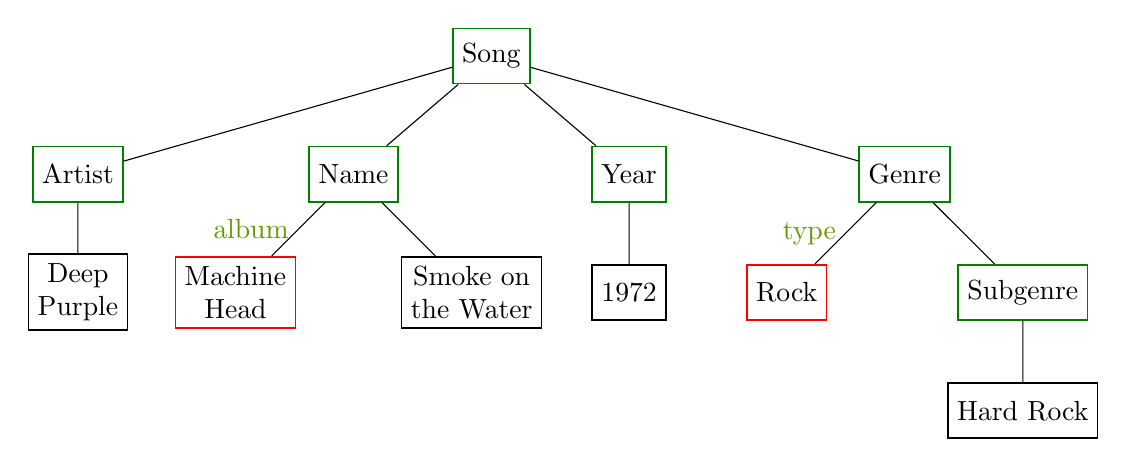
\begin{tikzpicture}[level distance=1.5cm,
  level 1/.style={sibling distance=3.5cm},
  level 2/.style={sibling distance=3cm},
  element/.style={ draw=black!50!green, fill=white, semithick, minimum size=7mm, align=center},
  attribute/.style={ draw=red, fill=white, semithick, minimum size=7mm, align=center},
  textnode/.style={ draw=black, fill=white, semithick, minimum size=7mm, align=center}]
  \node [element]{Song}
    child {node [element]{Artist}
      child {node [textnode]{Deep \\ Purple}}
    }
    child {node [element]{Name}
      child {node [attribute]{Machine \\ Head} edge from parent node[left, color=green!60!red]{album}}
      child {node [textnode]{Smoke on \\ the Water}}
    }
    child {node [element]{Year}
      child {node [textnode]{1972}}
    }
    child {node [element]{Genre}
      child {node [attribute]{Rock} edge from parent node[left, color=green!60!red]{type}}
      child {node [element]{Subgenre}
        child {node [textnode]{Hard Rock}}
      }
    };
\end{tikzpicture}
  \label{fig:xml_tree_intro}

\caption{XML-Datei und zugehöriger Baum}
\label{fig:xml_intro}
\end{figure}

Darüber hinaus existieren noch weitere Knotentypen wie Kommentare oder CDATA-Abschnitte, wobei letztere eine Sonderform des Textknotens sind und auch sonst für Markup reservierte Zeichen erlauben \autocite[Abs. 2.7]{xmlSpec}. 

Zuletzt sollen noch kurz die Begriffe der \textit{Wohlgeformtheit} und der \textit{Validität} eingeführt werden. Ein XML-Dokument ist dann wohlgeformt, wenn alle Regeln gemäß der Definition der W3C in dem Dokument eingehalten werden. Diese beinhalten u.\,a., dass es wie zuvor erwähnt nur ein Wurzelelement gibt oder dass jedes geöffnete Tag <\textit{Elementname}> auch ein schließendes Tag </\textit{Elementname}> besitzt \autocite[Abs. 2.1]{xmlSpec}.

Ein valides XML-Dokument muss wohlgeformt sein, einer Grammatik zugehörig sein und diese auch einhalten. Mögliche Formen dieser Grammatiken sind Dokumenttypdefinitionen (DTD) und XML-Schemadefinitionen (XSD)\autocite[Abs 2.8]{xmlSpec}\autocite[Abs 2.1]{xsdSpec}. 

\subsection{JavaScript Object Notation}

\acrfull{json} ist ein weiteres textbasiertes Datenformat, welches auf einer hierarchischen Datenstruktur basiert und dadurch als Baumstruktur betrachtet werden kann. Es ist dadurch in bestimmten Aspekten ähnlich zu XML, wobei es aber distinkte Unterschiede gibt. 

Jedes JSON-Dokument beginnt mit einem Wurzelknoten, welches anders als in XML keinen eigenen Namen hat und damit ausschließlich Informationen zu den eigenen Kindknoten beinhaltet. Für diese Kindknoten existieren im Wesentlichen 3 verschidene Knoten- bzw. Elementtypen:

\begin{description}
\item[Value-Knoten]
Die einfachste Form in JSON Daten zu speichern, ist in einem einzigen Key-Value Paar. Der Key ist dabei ein auf der aktuellen Ebene eindeutiger Identifier, welcher innerhalb von doppelten Anführungszeichen steht und von einem Doppelpunkt gefolgt wird. Das Value kann ein Integer-, Boolean-, String- oder Null-Wert sein \autocite[]{jsonSpec}. Für Strings besteht die Besonderheit, dass dort das Value auch in doppelten Anführungszeichen stehen muss.
\item[Array-Knoten]
Ein JSON-Array ist eine geordnete Liste an beliebigen Elementtypen, die jeweils durch Kommata getrennt sind \autocite[]{jsonSpec}. Ein Array hat auch genau einen für die Ebene eindeutigen Key und die Value-Elemente werden über ihren Index im Array adressiert. Diese Elementliste beginnt mit einem \glqq $[$ \grqq{} und endet mit einem \break\glqq $]$ \grqq{}.
\item[Objekt-Knoten]
Ein JSON-Objekt wird ebenfalls über einen eindeutigen Key adressiert. Es beinhaltet eine ungeordnete Liste an Elementen, welche wie beim Array durch Kommata getrennt sind. Anders als beim Array ist jedes Element innerhalb eines Objekts ein Key-Value Paar, und wird über den Key adressiert. Die Elemente eines JSON-Objekts sind durch \glqq \{ \grqq{} bzw. \glqq \} \grqq{} begrenzt.
\end{description}

Im Vergleich zu XML fehlt also die Unterstützung für Attribute und Kommentare als Knotentyp. Häufig lassen sich dennoch Informationen aus einer XML-Darstellung in JSON übersetzen. Dies ist hier beispielhaft für die XML-Datei aus Abb. \ref{fig:xml_intro} geschehen. 

\begin{figure}[!htb]
\begin{minted}{json}
{
    "Artist": "Deep Purple",
    "Name": {
       "Album": "Machine Head",
       "Name": "Smoke on the Water"
    },
    "Year": 1972,
    "Genre": {
       "Type": "Rock",
       "Subgenre": ["Hard Rock"]
    }
 }
\end{minted}
\caption{JSON-Datei analog zu Abb. \ref{fig:xml_intro}}
\label{fig:json_intro}
\end{figure}

Analog zu XML existieren die Begriffe der Wohlgeformtheit und Validität auch für JSON. Für valide JSON-Dateien existieren JSON-basierte Schemata gegen die diese Dateien geprüft werden. Außerdem muss eine valide JSON-Datei wohlgeformt sein und darf dadurch keine strukturellen Fehler beinhalten.

\newpage
\subsection{Java}
Java ist eine vielseitige, objektorientierte und weit verbreitete Programmiersprache. Laut \autocite{tiobe} gehört Java auch aktuell noch zu den 3 beliebtesten Programmiersprachen nach C und Python. Im Folgenden werden Java-spezifische Aspekte, die für das Projekt relevant sind, kurz aufgeführt. 

\subsubsection{Verwendete Libraries}

Für die Entwicklung einer Software mit mehreren Funktionen ist es häufig von Vorteil, bereits geschriebenen Code von reputablen Quellen wiederzuverwenden. Im Kontext von Java ist es möglich, fremden Code in Form von Libraries zu verwenden. Zu den zugehörigen Vorteilen gehört zum einen die Zeitersparnis, da der Code nicht neu entwickelt werden muss und zum anderen die Qualität des Codes. Häufig sind Libraries Open-Source, wodurch jeder Entwickler die Möglichkeit hat Fehler zu finden und zu melden oder diese direkt zu beheben. 

Bei der Entwicklung von MultiTextCompare wurden deshalb mehrere Libraries verwendet. 

\paragraph{JDOM}\mbox{}\\
JDOM bietet eine breit aufgestellte API zur Verarbeitung von XML-Dateien. In MultiTextCompare wird JDOM verwendet um XML-Dateien auf Wohlgeformtheit und Validität zu prüfen, um sie bspw. durch Sortierung zu manipulieren und um ihre XML-Strukturbäume für den Vergleich zu nutzen. Für die Validierung enthält JDOM einen Parser, der die Dateien zunächst nur auf Wohlgeformtheit prüft. Je nach Konfiguration ist es auch möglich, die Dateien über DTDs und XSDs zu validieren. Für das Traversieren der Dokumentbäume bzw. des \acrfull{dom} liefert JDOM die Klassen \textit{Element} und \textit{Attribute}. Dabei ist es für jedes Element möglich, dessen Kindelemente und Attribute zu erfragen.

\paragraph{Jackson}\mbox{}\\
Analog zu JDOM und XML bietet Jackson eine API für die Verarbeitung von JSON-Dateien. Die Aufgaben der API im Projekt sind nahezu identisch, wobei hier die Validierung wegfällt. Auch über Jackson lässt sich das \acrshort{dom} erzeugen und navigieren. Dafür existiert die Klasse \textit{JsonNode} mit welcher sich die Kindknoten eines Elements auflisten lassen.

\paragraph{Apache Commons}\mbox{}\\
Apache Commons ist eine Bibliothekssammlung von frei verfügbaren Java-Klassen. Für das Projekt wird die Implementierung der Levenshtein-Distanz, LCS-Länge und \acrshort{diff} innerhalb von \textit{apache.commons.text} verwendet, sowie einige dateibezogene Utility-Methoden aus der Bibliothek \textit{apache.commons.io}.

\subsubsection{Nebenläufigkeit}

Java bietet Entwicklern die Möglichkeit, die Ausführung ihrer Software zu parallelisieren. Konkret passiert das über das Konzept von Threads, also die mögliche Aufteilung von Aufgaben eines zugehörigen Prozesses auf kleinere Teilstücke. Falls keine Parallelisierung stattfindet, existiert pro Prozess genau ein Thread. Prozesse und Threads werden vom Betriebssystem bzw. vom Scheduler des Betriebssystems verwaltet, wobei Java über die Klasse \textit{Thread} Methoden bereitstellt, um Programme aufzuteilen und auf mehrere Threads zu verteilen. Das sog. \textit{Multithreading} hat besonders für Mehrkernprozessoren Vorteile, da die ausgeführte Java-Anwendung so mehrere Prozessorkerne gleichzeitig belasten kann, anstatt alle Aufgaben sequentiell auf einem Prozessorkern abzuarbeiten. Dies kann zu einer erheblichen Verbesserung der Bearbeitungszeit führen.

\subsubsection{Java Swing}

Java Swing ist ein \acrshort{ui}-Toolkit, welches gängige \acrshort{ui}-Komponenten in Form von Java Klassen realisiert und für die Entwicklung zur Verfügung stellt. Dazu gehören u.\,a. Buttons, Textfelder und Labels, die in nahezu jeder Anwendung mit Benutzerinteraktion vorhanden sind. 

Swing ist durch die Vielseitigkeit und Modularität der Komponenten zwar auf der Oberfläche relativ simpel aufgebaut, allerdings gibt es ein paar Besonderheiten im Zusammenhang mit Threads. Für das Event-Handling existiert in Swing der \acrfull{edt}. Wird bspw. ein Button vom Benutzer gedrückt, so wird die dem Button zugehörige Handler-Methode aufgerufen und auf dem \acrshort{edt} ausgeführt \autocite[]{edtDocs}. Für die Ausführungsdauer dieser Handler-Methode ist der \acrshort{edt} dann blockiert und es kann nicht auf weitere Benutzereingaben reagiert werden. 
Um dennoch Methoden mit langer Ausführdauer aus der \acrshort{ui} aufrufen zu können, existiert die Java Klasse \textit{SwingWorker}, die zwei überladene Methoden \textit{doInBackground()} und \textit{done()} zur Verfügung stellt. Für \textit{doInBackground()} wird ein separater Worker-Thread erstellt, auf dem dann die lang andauernden Methoden laufen während der \acrshort{edt} weiterhin auf Benutzereingaben reagiert. Erst sobald der Worker-Thread beendet ist, wird die \textit{done()}-Methode ausgeführt \autocite[]{swingWorkerDocs}.
Ein weiteres, wichtiges Detail ist, dass UI-Komponenten in Swing nicht thread-safe sind. Falls also zwei Threads gleichzeitig auf eine Komponente zugreifen, führt dies zu undefiniertem Verhalten. Dadurch gilt es als \textit{best practice} UI-Komponenten nur über den \acrshort{edt} zu manipulieren \autocite[]{edtDocs}. Im Kontext von SwingWorker, sollten jegliche UI-Zugriffe nur über die \textit{done()}-Methode ausgeführt werden, da diese auf dem \acrshort{edt} ausgeführt wird.